\documentclass[conference]{IEEEtran}
\IEEEoverridecommandlockouts
% The preceding line is only needed to identify funding in the first footnote. If that is unneeded, please comment it out.
\usepackage{cite}
\usepackage{amsmath,amssymb,amsfonts}
\usepackage{algorithmic}
\usepackage{graphicx}
\usepackage{textcomp}
\usepackage{xcolor}
\usepackage{amsmath}
\usepackage{minted}
\usepackage{float}
\usepackage[hyphens]{url}
\def\BibTeX{{\rm B\kern-.05em{\sc i\kern-.025em b}\kern-.08em
    T\kern-.1667em\lower.7ex\hbox{E}\kern-.125emX}}
\begin{document}

\title{Credit Card Fraud Detection\\}

\author{\IEEEauthorblockN{Duarte Mortágua}
\IEEEauthorblockA{\textit{DETI, UA} \\
\textit{Universidade de Aveiro}\\
Aveiro, Portugal \\
Número Mecanográfico: 92963}
\and
\IEEEauthorblockN{Mário Silva}
\IEEEauthorblockA{\textit{DETI, UA} \\
\textit{Universidade de Aveiro}\\
Aveiro, Portugal \\
Número Mecanográfico: 93430}
}

\maketitle

\begin{abstract}
Credit card frauds happen every day alongside millions of other normal transactions. The gigantic amount of apparently similar transactions obfuscates fraudulent transactions in financial institutions. Although they represent less than 1\% of the total transactions, they can cause significant damage. Businesses face legal problems by not being able to detect and avoid these transactions. Adaptive and modern machine learning models and algorithms are the answer to this problem.
\end{abstract}
\begin{IEEEkeywords}
Machine Learning, Credit Card Fraud Detection, Classification Problem, Imbalanced Data
\end{IEEEkeywords}


\section{Introduction}
This report was made to demonstrate our apprenticeships and explain the reasons behind our decisions and thought process during the investigation phase of this project and throughout the course of TAA - Tópicos de Aprendizagem Automática.

The goal of this project is to design, implement and compare some machine learning models that can detect fraudulent credit card transactions.

In financial institutions, thousands of credit or debit card transactions are performed every second. The difficulty of fraud detection is increased by the large volume of data and its natural sequential structure. The majority of production-level analytical strategies still rely on batch learning, which is insufficient for two reasons: Models quickly become obsolete, requiring the storage of sensitive data. The ever-changing nature of bank fraud emphasizes the significance of having up-to-date models, and the retention of sensitive data exposes businesses to violations of the European General Data Protection Regulation. For these reasons, it's a good idea to develop modern, adaptive, and accurate machine learning models in this field.


\section{State-Of-The-Art analysis}

After analyzing the most relevant content and discussions about the topic of fraudulent credit card transactions, multiple conclusions were made about the methods that take concerns to the data processing and the machine learning model itself. 

Most of the transactions were Non-Fraud (99.83\%) of the time, while Fraud transactions occur (0.17\%) of the time. Due to this fact, some authors agree that a good solution should be to create a sub-sample with a 50/50 ratio of fraud and non-fraud transactions \cite{paper_sqewed_data_calssifier}\cite{paper_dealing_with_imbalanced}. This can be achieved by over-sampling or under-sampling. Most of the works done under this context tend to use over-sampling \cite{paper_sqewed_data_calssifier}\cite{paper_dealing_with_imbalanced} for one simple reason: Under-sampling causes the loosing of a large amount of data, which leads to low precision. More specifically, some authors use a particular over-sampling approach: SMOTE - Synthetic Minority Over-sampling Technique.

It is highly recommendable to do the over-sampling during cross-validation, instead of before. This is because doing over-sampling before cross-validation directly influences the validation, causing a "data leakage" problem \cite{paper_dealing_with_imbalanced}.

Some authors have also detected anomalies in the dataset (outliers), and defend that their removal is mandatory. Some works detect and remove the outliers just by visualizing the data, while others defend more elaborated approaches like using the Winsorization Method or Percentile Capping \cite{paper_outlier_silent_killer}.

The most used classifier is Logistic Regression \cite{paper_sqewed_data_calssifier}\cite{paper_imbalanced_detail}\cite{paper_dealing_with_imbalanced}, which some authors defend as revealing the best Receiving Operating Characteristic score (ROC), meaning that Logistic Regression accurately separates fraud and non-fraud transactions. Some authors also used the Random Forest classifier, but it later revealed to cause over-fitting.

Simple Logistic Regression Models with no sampling are also used but often lead to inaccurate results due to the simplicity of the model alone \cite{paper_simple_logistic}.

Even simpler models are presented, using Autoencoders and Unsupervised Learning for example \cite{paper_autoencoders}. By decomposing the original dataset with the T-SNE (t-Distributed Stochastic Neighbor Embedding) technique, a dataset with reduced dimensions is produced containing only the top n components with maximum information. Then, the autoencoder is trained and achieves high accuracy levels. On the other hand, some authors suspect data leakage and overfitting related to this model.

In terms of metrics, some authors defend not using accuracy score as a metric with imbalanced datasets like this one (will be usually high and misleading), instead use f1-score, precision/recall score or even confusion matrix \cite{paper_dealing_with_imbalanced}.

\section{Machine Learning Problem Complexity}

This problem of classifying transactions contains thirty features. There are a lot of other problems which a higher number of features, however, thirty is still is a considerable amount and it still may lead to overfitting with this amount of features. Also, dealing with an imbalanced dataset is a tough challenge in machine learning, which increased this problem complexity a lot more.

To solve this problem we chose a linear model, logistic regression, but also tested with a nonlinear one, k-nearest neighbors. They both have simple algorithmic complexity, however, the k-nearest neighbors model is more computationally expensive than the other.

\section{Data Description}

The datasets contain transactions made by credit cards in September 2013 by European cardholders. Also, it presents transactions that occurred in two days, where there are 492 frauds out of 284,807 transactions. The dataset is highly unbalanced, the positive class (frauds) account for 0.172\% of all transactions.

\begin{figure}[H]
    \centerline{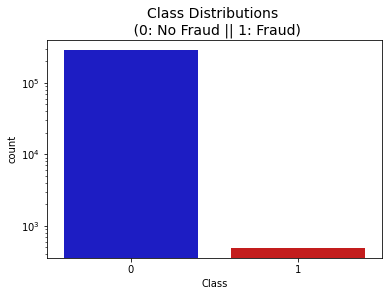
\includegraphics[width=0.5\textwidth]{images/class_distribution.png}}
    \caption{Class Distribution}
    \label{fig:hist_test_classes}
\end{figure}

Twenty-eight features don't have their original name and don't provide more background information about the data due to confidentiality issues and all of these (V1, V2, ..., V28) features were all previously scaled and then transformed with PCA. PCA is defined as an orthogonal linear transformation that transforms the data to a new coordinate system such that the greatest variance by some scalar projection of the data comes to lie on the first coordinate (called the first principal component), the second greatest variance on the second coordinate, and so on it is a method used to reduce the number of variables in the data by extracting important one from a large pool. It reduces the dimension of the data to retain as much information as possible.

It is worth mentioning that to implement a PCA transformation features need to be previously scaled. In our case, all the V features have been scaled (or at least that is what we presume the people that develop the dataset did).

The other 2 features, Time and Amount, did not go through a PCA transformation. Feature Time contains the seconds elapsed between each transaction and the first transaction in the dataset. The feature Amount is the transaction Amount, this feature can be used for example-dependant cost-sensitive learning, the transactions' amounts are relatively small. The mean of all the mounts made is approximately USD 88.

There are no "Null" values, so we don't have to work on ways to replace values.

Finally, there is a label Class in the last column of each row that is the response variable and it takes value 1 in case of fraud and 0 otherwise.

\subsection{Statistical Analysis}

As mentioned before, the distribution of the credit card transactions in the dataset is not uniform. This would be a problem if the train set had the same kind of distribution, meaning that there would be more classes of one type than the other. Working with this biased data could lead to misjudging relatively to our model results, and could also be problematic when creating our cross-validation subset more ahead.

\begin{figure}[!htpb]
    \centerline{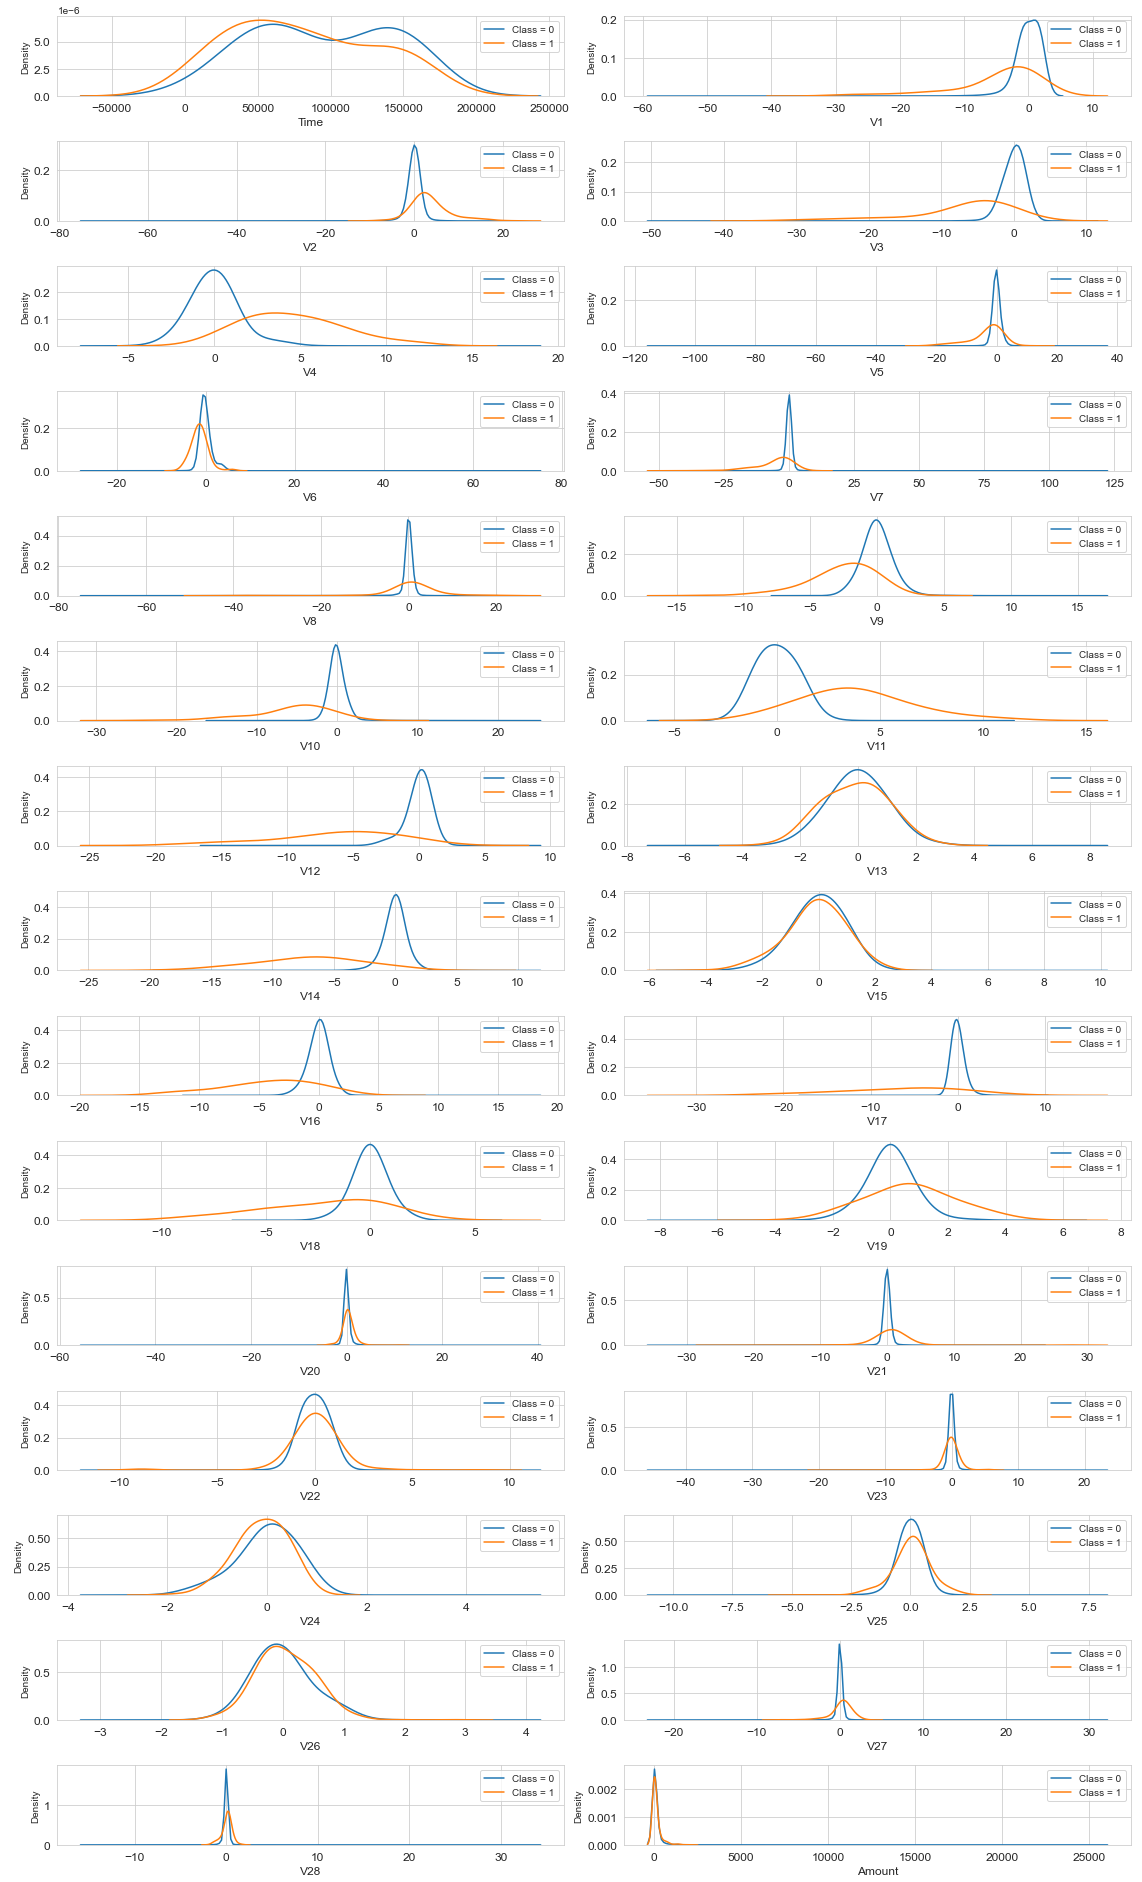
\includegraphics[width=0.5\textwidth]{images/feature_values.png}}
    \caption{Feature Values}
    \label{fig:feat_values}
\end{figure}

From the figure \ref{fig:feat_values} we can visualize that a lot of features have values around 0 on normal transactions, and, on fraudulent ones, they tend to deviate a little from their normal values. Other features, for example, V15, have similar values in both cases.

\section{Data Processing And Analysis}

\subsection{Scaling the data}

As we know, all the features were already scaled and submitted to a PCA transformation, except for the Time and Amount, which need to be scaled.

Scaling was achieved by using a RobustScaler \cite{sklearn_robust_scaler}. This Scaler removes the median and scales the data according to the quartile range, resulting in being less prone to outliers.

\begin{table}[H]
\caption{A. Amount and Time features before scaling}
\begin{center}
\begin{tabular}{|c|c|c|c|}
\hline
\textbf{} & \textbf{amount} & \textbf{time}& \textbf{V1} \\
\hline
0 & 149.62 & 0.0 & -1.359807 \\
1 & 2.69 & 0.0 & 1.191857 \\
2 & 378.66 & 1.0 & -1.358354 \\
3 & 123.50 & 1.0 & -0.966272 \\
\hline
\end{tabular}
\end{center}
\end{table}

\begin{table}[H]
\caption{A. Amount and Time features after scaling}
\begin{center}
\begin{tabular}{|c|c|c|c|}
\hline
\textbf{} & \textbf{amount} & \textbf{time}& \textbf{V1} \\
\hline
0 & 1.783274 & -0.994983 & -1.359807 \\
1 & -0.269825 & -0.994983 & 1.191857 \\
2 & 4.983721 & -0.994972 & -1.358354 \\
3 & 1.418291 & -0.994972 & -0.966272 \\
\hline
\end{tabular}
\end{center}
\end{table}

\subsection{Splitting the data}
The data was split into train and test by using the \textit{StratifiedKFold} library \cite{sklearn_strat_kfold}. This cross-validation object is a variation of KFold that returns stratified folds. The folds are made by preserving the percentage of samples for each class. Since we're dealing with an imbalanced class distribution (that should remain that way until testing our model), we chose \textit{StratifiedKFold} over \textit{KFold}.

The preservation of the data was tested and confirmed right after the splitting, by counting the labels and obtaining its percentages in the dataset.

\subsection{Balancing the data}
As mentioned before, this dataset has the peculiarity of being highly unbalanced, meaning that most of the cases are non-fraud. Using the dataset as it is would cause overfit since the model will assume that most of the transactions are non-fraud.

Our algorithm will only understand relevant patterns if it has enough fraud and non-fraud examples to sustain it, enough meaning an equal (or close to equal) amount of both cases.

Since we have such few fraud cases to so many non-fraud cases, we decided to create a sub-sample of the given data, with a  50/50 ratio of fraud and non-fraud transactions.
We accomplished this by combining the 492 examples of fraud (all) with 492 randomly selected non-fraud cases, an action that was proceeded by shuffling the data.

\begin{figure}[H]
    \centering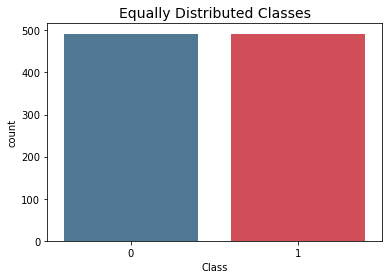
\includegraphics[width=0.5\textwidth]{images/classes_after_balancing.png}
    \caption{Class Distribution after balancing}
    \label{fig:example}
\end{figure}

\subsection{Correlating}
The next step in data analysis is understanding the features. Just by looking, 30 features with normalized values don't reveal much information.

Correlation matrices are the essence of understanding our data, which helps us know if there are features that influence heavily the type of the transaction.

We must use the correct data frame (subsample) for us to see which features have a high positive or negative correlation concerning fraud transactions.

\begin{figure}[H]
    \centering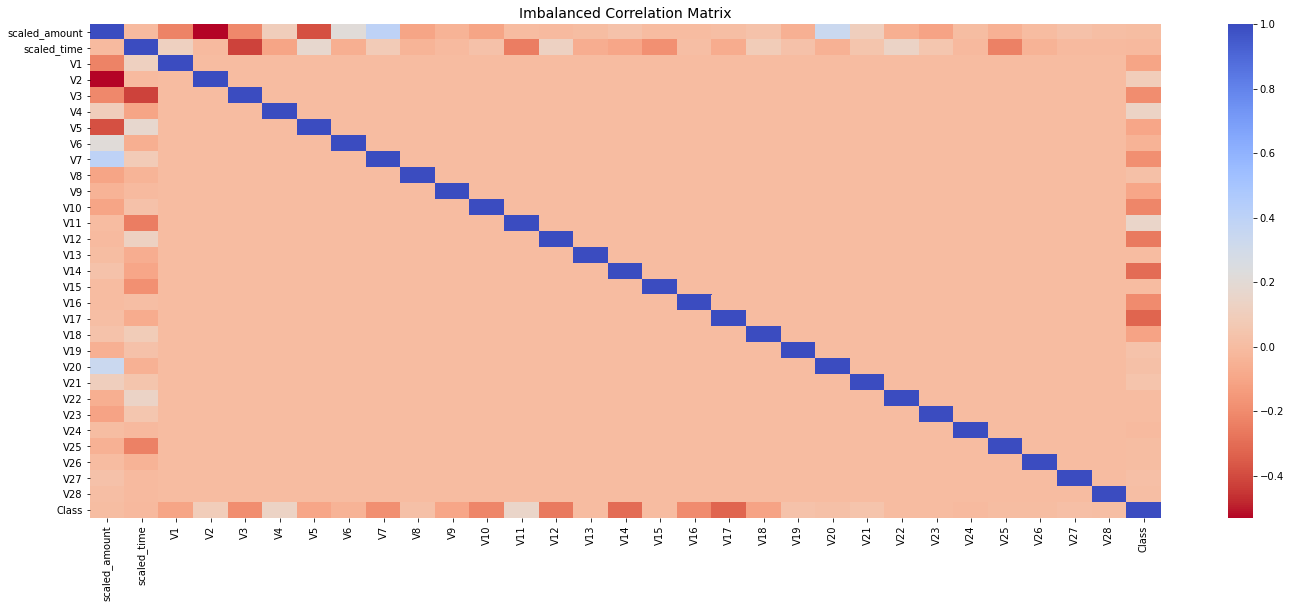
\includegraphics[width=0.5\textwidth]{images/imbalanced_corr_matrix.png}
    \caption{Correlation matrix using the imbalanced dataset (all)}
    \label{fig:example}
\end{figure}

\begin{figure}[H]
    \centering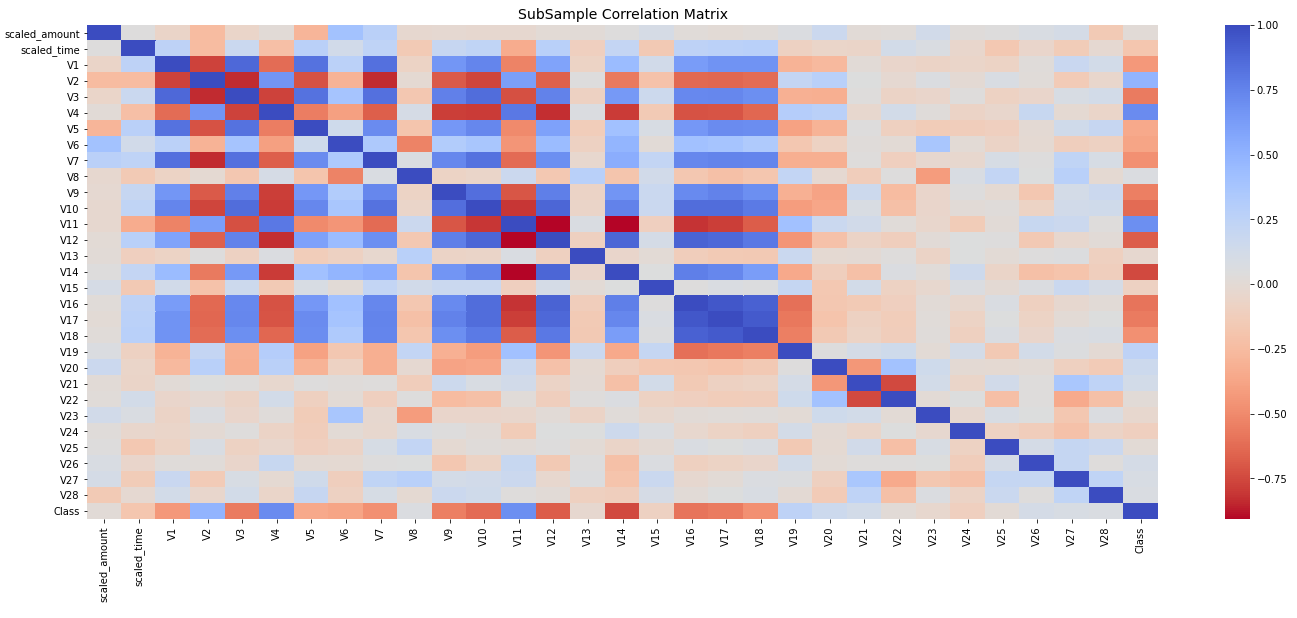
\includegraphics[width=0.5\textwidth]{images/balanced_corr_matrix.png}
    \caption{Correlation matrix using the balanced dataset (sub-sample)}
    \label{fig:correlation_sub}
\end{figure}

By analyzing the results on the balanced dataset, we can spot negative correlations and positive correlations \cite{paper_dealing_with_imbalanced}.
For example, V17, V14, V12, and V10 are negatively correlated, since the lower these values are, the more likely the result will be a fraud transaction. On the other hand, V2, V4, V11, and V19 are positively correlated, since the higher their values are, the more likely the result will be a fraud transaction.

\subsection{Visualizing clustered data}

T-Distributed Stochastic Neighbor Embedding (t-SNE) is an unsupervised, non-linear technique primarily used for data exploration and visualizing high-dimensional data.

T-SNE attempts to find the underlying structure of the data by taking into account the neighbors of a sample.
In simpler terms, t-SNE gives us a feel or intuition of how the data is arranged in a high-dimensional space. If the data looks linearly separable, it usually means that the predictive models will perform pretty well in separating fraud cases from non-fraud cases.

To follow the t-STE, we also tried some linear dimensionality reduction techniques: PCA and SVD.

\begin{figure}[H]
    \centering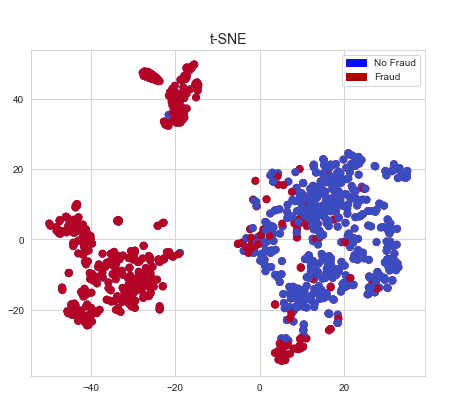
\includegraphics[width=0.4\textwidth]{images/clustering _tsne.png}
    \caption{Clustering data using t-SNE (non-linear dimensionality reduction)}
    \label{fig:example}
\end{figure}

\begin{figure}[H]
        \centering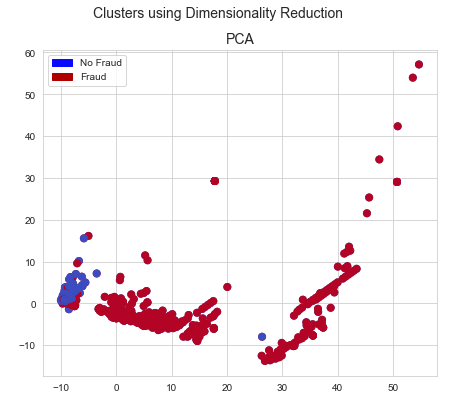
\includegraphics[width=0.4\textwidth]{images/clustering_pca.png}
    \caption{Clustering data using PCA (linear dimensionality reduction)}
    \label{fig:example}
\end{figure}

\begin{figure}[H]
        \centering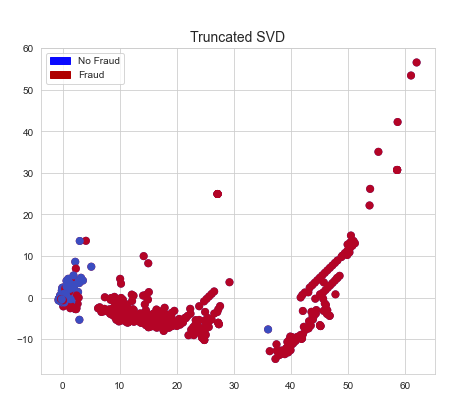
\includegraphics[width=0.4\textwidth]{images/clustering_svd.png}
    \caption{Clustering data using Truncated SVD (linear dimensionality reduction)}
    \label{fig:example}
\end{figure}

All the algorithms can detect clusters pretty accurately, meaning that the data is linearly separable.

\section{Model}

\subsection{Logistic Regression}
Logistic Regression is a type of analysis that is used if the goal is to determine the category/class of the output. It is a generalized linear model because the outcome always depends on the sum of the inputs and parameters. Or in other words, the output cannot depend on the product of its parameters.\cite{raschka}

Logistic regression was an obvious approach for us since it is usually recommended for problems when the classification can take only two values, and if the data is linearly separable because it is more efficient to classify it into two separate classes. Also, Logistic regression is much easier to implement than other methods. \cite{log_reg_def}

\subsection{K-Nearest Neighbors}

KNN is a non-parametric and lazy learning algorithm. Non-parametric means there is no assumption for underlying data distribution. In other words, the model structure is determined from the dataset. This will be very helpful in practice where most of the real-world datasets do not follow mathematical theoretical assumptions. A lazy algorithm means it does not need any training data points for model generation. All training data used in the testing phase. This makes training faster and the testing phase slower and costlier.\cite{knn_def}.

We opted for KNN as another model since the algorithm is simple, easy to implement, and very versatile since it can be used for classification, regression, and search problems. However, KNN gets significantly slower as the number of examples and/or predictors/independent variables increase, since our data is relatively big and we have a lot of features, it is extremely slow if we used the SMOTE technique, as we are going to explain in the next sections, for that reason we opted to use undersampling with this model.

\subsection{Hyperparameter Tuning Methods}

Searching for the right hyperparameters to obtain the highest precision and accuracy is considered to be one of the trickiest parts of building machine learning and artificial intelligence models, and, it is hard to scale for high dimensional data because of the increase of the number of iterations, which in turn expands the training time \cite{hyper_parameters}.

There are several parameter tuning techniques, but we opted for two of the most widely-used parameter optimizer techniques:

\begin{itemize}
\item \textbf{Grid search}: \\
Grid search is an exhaustive search for selecting a model. In Grid Search, the data scientist sets up a grid of hyperparameter values and for each combination, trains a model and scores on the testing data. In this approach, every combination of hyperparameter values is tried which can be very inefficient.
We decided to use this method with for the K-Nearest Neighbors model (we got better results with it), to find the best parameters out of the following "grid" defined by us: \\
knears\_params = {"n\_neighbors": list(range(2,5,1)), 'algorithm': ['auto', 'ball\_tree', 'kd\_tree', 'brute']}

\item \textbf{Randomized search}: \\
Randomized Search sets up a grid of hyperparameter values and selects random combinations to train the model and score. This allows to explicitly control the number of parameter combinations that are attempted. The number of search iterations is set based on time or resources. While it’s possible that Randomized Search will not find as accurate of a result as Grid Search, it surprisingly picks the best result more often than not and in a fraction of the time Grid Search would have taken. In our case, we passed these parameters to the Randomized Search: \\
log\_reg\_params = {"penalty": ['l1', 'l2'], 'C': [0.001, 0.01, 0.1, 1, 10, 100, 1000]} \\
We used this search for logistic regression because it was way faster and in the end, it also got better results.
\end{itemize}


\subsection{Cross-Validation}
Cross-validation is needed to avoid overfitting. We could get a good score without cross-validating but that would not necessarily mean that it would perform well with the test set. 

When building a machine learning model using some data, it is common to split the data into training and validation/test sets. The training set is used to train the model, and the validation/test set is used to validate it on data it has never seen before. The classic approach is to do a simple 80\%-20\% split. In cross-validation, it is done more than one split. It can be done 3, 5, 10, or any K number of splits. Those splits are called Folds. \cite{cross_val}

For our problem we used Stratified Cross-Validation as mentioned before, we split our data into 5 folds, and we want to each fold to be a good representative of the whole data, so, the proportion of normal and fraudulent classes must be similar in each fold, for this reason, we enforced a correct distribution.

\subsection{SMOTE}

Several different techniques exist in the practice for dealing with imbalanced datasets. The most naive class of techniques is sampling: changing the data presented to the model by undersampling common classes, oversampling (duplicating) rare classes, or both.

Undersampling means taking the less number of majority class (In our case taking less number of Normal transactions so that our new data will be balanced).

Oversampling means replicating the data of the minority class (fraud class) so that we can have balanced data.

SMOTE stands for Synthetic Minority Over-sampling Technique and is an oversampling technique. It creates synthetic points from the minority class in order, fraudulent class, to reach an equal balance between the minority and majority class. SMOTE picks the distance between the closest neighbors of the minority class, in between these distances it creates synthetic points.

\begin{figure}[H]
        \centering\includegraphics[width=0.5\textwidth]{images/SMOTE.png}
    \caption{Smote Technique}
    \label{fig:smote_tech}
\end{figure}

When oversampling the data, cross-validation shouldn't be done before cross-validating, because it will be directly influencing the validation set before implementing cross-validation causing a "data leakage" problem. In our case, when doing the cross-validation we take 4/5 of our set as a training set and 1/5 as our validation set. If we performed SMOTE before and then perform cross-validation we are testing on synthetic data points, but we want to test on real data. The goal of using SMOTE is to create similar data so our model can capture the pattern but the test set or validation set in this case cannot be touched. We want to see if our model is obtaining the patterns with more information through SMOTE to detect Fraud cases not synthetic generated, this way we also avoid overfitting.

\begin{figure}[H]
        \centering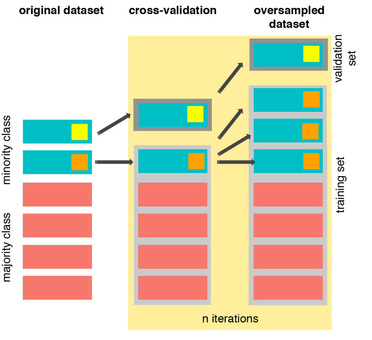
\includegraphics[width=0.5\textwidth]{images/smote_during_cv.jpeg}
    \caption{Smote During Cross-Validation}
    \label{fig:smote_cv}
\end{figure}

\section{Results}

We want to make sure that our model detects fraud cases, True Positives, and that it knows that a specific transaction is not a fraud case, True Negatives. (We wouldn't like our bank to block our cards when purchasing something because they believed the transaction was a fraud case.)

\begin{itemize}
\item True Positives: Correctly Classified Fraud Transactions
\item False Positives: Incorrectly Classified Fraud Transactions
\item True Negative: Correctly Classified Non-Fraud Transactions
\item False Negative: Incorrectly Classified Non-Fraud Transactions
\end{itemize}


\subsection{Precision and Recall}

\begin{center}
  \begin{equation} \label{eq:precision}
    P = \frac{TP}{TP + FP}
  \end{equation}
  P: Precision \\
  TP: True Positives \\
  FP: False Positives
\end{center}

\begin{center}
  \begin{equation} \label{eq:recall}
    R = \frac{TP}{TP + FN}
  \end{equation}
  R: Recall \\
  TP: True Positives \\
  FN: False Negatives
\end{center}

Precision as the name says, says how precise our model is in detecting fraudulent transactions while recall is the number of fraud cases our model can detect.

The precision-recall curve shows the tradeoff between precision and recall for different thresholds. A high area under the curve represents both high recall and high precision, where high precision relates to a low false-positive rate, and high recall relates to a low false-negative rate \cite{sklearn_prec_rec}.

\begin{figure}[H]
    \centering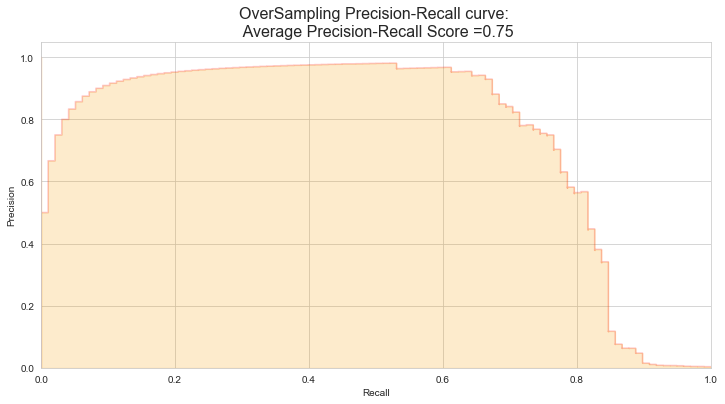
\includegraphics[width=0.5\textwidth]{images/prec_rec.png}
    \caption{Logistic Regression Precision-Recall Curve}
    \label{fig:prec_rec}
\end{figure}

For the logistic regression model, precision starts to descend between 0.90 and 0.92 nevertheless, our precision score is still pretty high and with a decent recall score.

\subsection{ROC And AOC}

A ROC curve (receiver operating characteristic curve) is a graph showing the performance of a classification model at all classification thresholds \cite{roc_auc}. This curve plots two parameters:

\begin{itemize}
\item True Positive Rate, which is a synonym for recall, and can be calculated from the equation \ref{eq:recall}.
\item False Positive Rate, which can be calculated from the equation \ref{eq:fpr}.
\end{itemize}

\begin{center}
  \begin{equation} \label{eq:fpr}
    FPR = \frac{FP}{FP + TN}
  \end{equation}
  FPR: False Positive Rate \\
  FP: False Positives \\
  TN: True Negatives
\end{center}

A ROC curve plots TPR vs. FPR at different classification thresholds. Lowering the classification threshold classifies more items as positive, thus increasing both False Positives and True Positives. The following figure shows a typical ROC curve.

AUC stands for "Area under the ROC Curve." That is, AUC measures the entire two-dimensional area underneath the entire ROC curve (think integral calculus) from (0,0) to (1,1) \cite{roc_auc}.

\begin{figure}[H]
    \centering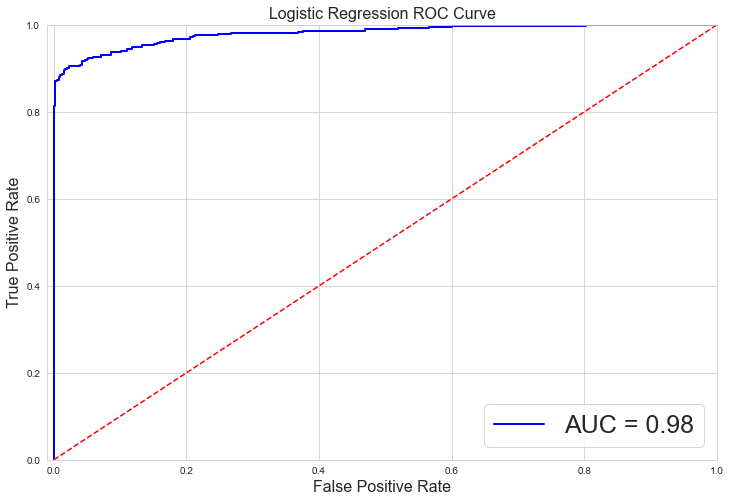
\includegraphics[width=0.5\textwidth]{images/roc_auc.png}
    \caption{Logistic Regression ROC Curve and AUC}
    \label{fig:roc_auc}
\end{figure}

\begin{figure}[H]
    \centering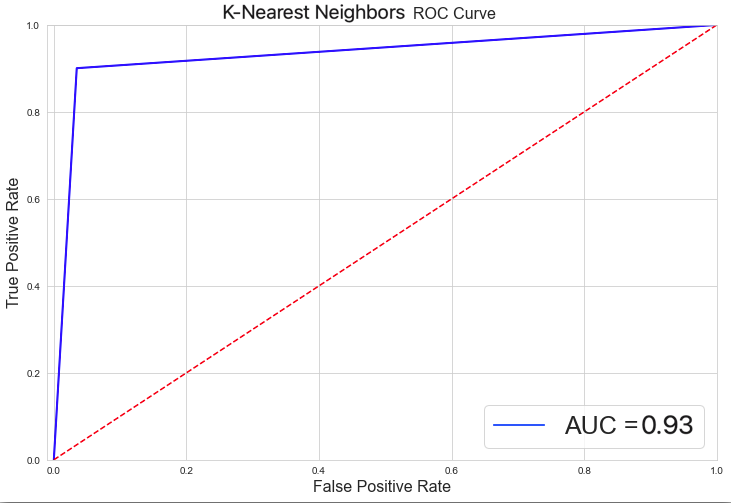
\includegraphics[width=0.5\textwidth]{images/roc_auc_kn.png}
    \caption{K-Nearest Neighbors ROC Curve and AUC}
    \label{fig:kn_roc_auc}
\end{figure}

Given we achieved an AUC of 0.98 with the logistic regression model, we believe this model has a good performance at distinguishing between the positive and negative classes, although, there are better ways to make sure, as we are going to show in the next section.

\subsection{Confusion Matrix}

One way to prove if the model is working precisely is through the confusion matrix because if we use an accuracy score we will get high scores since our model could just assume that all the cases are non-fraud cases that happen in 99.83\% of the cases. 

Using a confusion matrix on a sample that is balanced tells us how accurately it predicted both fraud and non-fraud cases which is more accurate than seeing the traditional accuracy score with imbalanced data sets.

On the top left-square, there are the True Negatives, this is the number of correctly classifications of the "No" (No Fraud Detected) class, and on the top-right square, there are the False Negatives, This is the number of incorrectly classifications of the "No"(No Fraud Detected) class.

On the bottom-left square, there are the False Positives, this is the number of incorrectly classifications of the "Yes" (Fraud Detected) class, and on the bottom-right square, there are the True Positives, this is the number of correctly classifications of the "Yes" (Fraud Detected) class.

\begin{figure}[H]
    \centering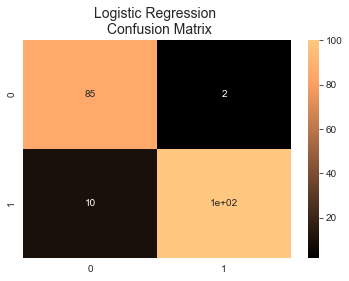
\includegraphics[width=0.5\textwidth]{images/lr_conf_matrix.png}
    \caption{Logistic Regression Confusion Matrix}
    \label{fig:lr_matrix}
\end{figure}

\begin{figure}[H]
    \centering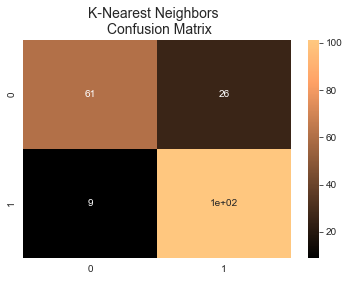
\includegraphics[width=0.5\textwidth]{images/kn_conf_matrix.png}
    \caption{K-Nearest Neighbors Confusion Matrix}
    \label{fig:kn_matrix}
\end{figure}

Comparing both confusion matrices, it is clear that the logistic regression model had more True Negatives and less False Negatives, meaning that it classified correctly transactions that weren't fraudulent more times than the K-nearest neighbors algorithm.

\subsection{Overall Accuracy}

From the same sample used for the confusion matrices, we were able to retrieve a classification report from both models:

\begin{table}[H]
\caption{Logistic Regression Classification Report}
\begin{center}
\begin{tabular}{|c|c|c|c|}
\hline
\textbf{} & \textbf{Precision} & \textbf{Recall}& \textbf{F1-Score} \\
\hline
0 (Normal) & 0.92 & 1.00 & 0.96 \\
1 (Fraud) & 1.00 & 0.93 & 0.96 \\
Accuracy & 0.96 & 0.96 & 0.96 \\
Macro Avg & 0.96 & 0.96 & 0.96 \\
Weighted Avg & 0.96 & 0.96 & 0.96 \\
\hline
\end{tabular}
\end{center}
\end{table}


\begin{table}[H]
\caption{K-Nearest Neighbors Classification Report}
\begin{center}
\begin{tabular}{|c|c|c|c|}
\hline
\textbf{} & \textbf{Precision} & \textbf{Recall}& \textbf{F1-Score} \\
\hline
0 (Normal) & 0.87 & 0.70 & 0.78 \\
1 (Fraud) & 0.80 & 0.92 & 0.85 \\
Accuracy & & & 0.82 \\
Macro Avg & 0.83 & 0.81 & 0.81 \\
Weighted Avg & 0.83 & 0.82 & 0.82 \\
\hline
\end{tabular}
\end{center}
\end{table}

The f1-score is the weighted average of Precision and Recall (Equation \ref{eq:f1score}). Therefore, this score takes both false positives and false negatives into account. F1-score is usually more useful than accuracy, especially with uneven class distributions. Accuracy works best if false positives and false negatives have similar costs. If the cost of false positives and false negatives are very different, it’s better to look at both Precision and Recall \cite{ex_f1_score}.

\begin{center}
  \begin{equation} \label{eq:f1score}
    F1 = 2*\frac{R * P}{R + P}
  \end{equation}
  F1: F1-Score \\
  R: Recall \\
  P: Precision
\end{center}

We also measured the accuracy with the entire test sample and got some high accuracies (Table \ref{tab:ov_acc}), which can be very misleading as stated previously.

\begin{table}[H]
\caption{Overall Accuracy}
\label{tab:ov_acc}
\begin{center}
\begin{tabular}{|c|c|}
\hline
\textbf{Technique} & \textbf{Accuracy} \\
\hline
Logistic Regression with Oversampling (SMOTE) & 0.986096\% \\
K-Nearest Neighbors with Undersampling & 0.780973\% \\
\hline
\end{tabular}
\end{center}
\end{table}

\section{Novelties and Contributions}

As it was stated in the beginning of this report, many authors refer to the removal of outliers as an effective data processing step to increase accuracy, more specifically "extreme outliers" from features that have a high correlation with our classes.

An outlier is an observation that is numerically distant from the rest of the data or in simple words it is the value that is out of the range.

The removal of outliers has to be done with caution. The lower the threshold, the more outliers it will remove, but we might run the risk of information loss which will cause our model to have lower accuracy.

In order to apply the outlier removal only in the features that are relevant for classification, we will choose only the features that are most correlated with our classes, according to our correlation matrix (Fig. \ref{fig:correlation_sub}), which are V10, V12, and V14.

Using a method mentioned the Winsorization (Percentile Capping) method (referenced as the best for the case \cite{paper_outlier_silent_killer}) to remove the "extreme outliers", and after choosing a threshold (1.5), the values of these features were truncated by respective 25 and 75 percentile.

As a result, our model (that was already at 98.6\% score) scored roughly the same.

We could have experimented with more threshold values to see if some threshold would increase our overall score, but as that would take some time and our score is already excellent, we left it that way.

\section{Conclusions and Future Work}

In this report, we have implemented techniques to process this dataset, such as scaling, splitting, and balancing. We have visualized our data through correlation matrices and dimensional reduction techniques. In the end, we have tested two different machine learning approaches to detect credit card fraud cases: logistic regression with SMOTE (oversampling), and k-nearest neighbors with undersampling.

The model which shows the best performance is Logistic Regression, which goes along with what other authors have already stated in prior works with this dataset. This model also shows a higher AUC than the k-nearest neighbors model algorithm, according to the calculated ROC curves.

We attempted an "extreme outliers" removal, as suggested by multiple authors, but it did not affect any of the models' performance. Future work can be done by varying the methods to remove the outliers and their parameters since we only tried one method with one parameter.

Although the Logistic Regression model has excellent results, future work can be done to improve, such as attempted other classifiers like SVM, Random Forest, Neural networks, or even Semi-Supervised methods like Autoencoders.

\begin{thebibliography}{00}

% Dataset
\bibitem{kaggle_dataset} Machine Learning Group - ULB. (2018, March 23). Credit Card Fraud Detection. Kaggle. \url{https://www.kaggle.com/mlg-ulb/creditcardfraud}

% Papers
\bibitem{paper_outlier_silent_killer} N. (2021, March 14). Outlier!!! The Silent Killer. Kaggle. \url{https://www.kaggle.com/nareshbhat/outlier-the-silent-killer}

\bibitem{paper_autoencoders} S. (2019, January 18). Semi Supervised Classification using AutoEncoders. Kaggle. \url{https://www.kaggle.com/shivamb/semi-supervised-classification-using-autoencoders}

\bibitem{paper_lre} G. (2021a, June 29). CreditCard Fraud Detection by Logistic Regression. Kaggle. \url{https://www.kaggle.com/gauravduttakiit/creditcard-fraud-detection-by-logistic-regression\#Interpreting-the-results:-Odds-Ratio,-Confidence-Intervals-and-Pvalues}

\bibitem{paper_dealing_with_imbalanced} J. (2019a, July 3). Credit Fraud - Dealing with Imbalanced Datasets. Kaggle. \url{https://www.kaggle.com/janiobachmann/credit-fraud-dealing-with-imbalanced-datasets}

\bibitem{cross_val} Shulga, D. (2018, September 27). 5 Reasons why you should use Cross-Validation in your Data Science Projects. Medium. \url{https://towardsdatascience.com/5-reasons-why-you-should-use-cross-validation-in-your-data-science-project-8163311a1e79}

\bibitem{paper_imbalanced_detail} G. (2017, May 30). How To handle Imbalance Data : Study in Detail. Kaggle. \url{https://www.kaggle.com/gargmanish/how-to-handle-imbalance-data-study-in-detail/data}

\bibitem{paper_tensorflow_cnn} C. (2017a, March 29). Predicting Fraud with TensorFlow. Kaggle. \url{https://www.kaggle.com/currie32/predicting-fraud-with-tensorflow}

\bibitem{paper_sqewed_data_calssifier} J. (2016, December 17). In depth skewed data classif. (93\% recall acc now). Kaggle. \url{https://www.kaggle.com/joparga3/in-depth-skewed-data-classif-93-recall-acc-now}

\bibitem{paper_simple_logistic} G. (2021b, June 29). CreditCard Fraud Detection by Logistic Regression. Kaggle. \url{https://www.kaggle.com/gauravduttakiit/creditcard-fraud-detection-by-logistic-regression}

% Specific libraries
\bibitem{sklearn_tsne} sklearn.manifold.TSNE — scikit-learn 0.24.2 documentation. (n.d.). Scikit-Learn.Org. Retrieved June 30, 2021, from \url{https://scikit-learn.org/stable/modules/generated/sklearn.manifold.TSNE.html}

\bibitem{sklearn_svd} sklearn.decomposition.TruncatedSVD - scikit-learn 0.24.2 documentation. (n.d.). Scikit-Learn.Org. Retrieved June 30, 2021, from \url{https://scikit-learn.org/stable/modules/generated/sklearn.decomposition.TruncatedSVD.html}

\bibitem{sklearn_pca} sklearn.decomposition.PCA - scikit-learn 0.24.2 documentation. (n.d.). Scikit-Learn.Org. Retrieved June 30, 2021, from \url{https://scikit-learn.org/stable/modules/generated/sklearn.decomposition.PCA.html}

\bibitem{sklearn_prec_rec} Precision-Recall — scikit-learn 0.24.2 documentation. (n.d.). Scikit-Learn.Org. Retrieved June 30, 2021, from \url{https://scikit-learn.org/stable/auto_examples/model_selection/plot_precision_recall.html}

\bibitem{sklearn_strat_kfold} sklearn.model\_selection.StratifiedKFold — scikit-learn 0.24.2 documentation. (n.d.). Scikit-Learn.Org. Retrieved June 30, 2021, from \url{https://scikit-learn.org/stable/modules/generated/sklearn.model\_selection.StratifiedKFold.html}

\bibitem{sklearn_robust_scaler} sklearn.preprocessing.RobustScaler — scikit-learn 0.24.2 documentation. (n.d.). Scikit-Learn.Org. Retrieved June 30, 2021, from \url{https://scikit-learn.org/stable/modules/generated/sklearn.preprocessing.RobustScaler.html}

% Resources
\bibitem{medium_tsne} Violante, A. (2018, August 30). An Introduction to t-SNE with Python Example - Towards Data Science. Medium. \url{https://towardsdatascience.com/an-introduction-to-t-sne-with-python-example-5a3a293108d1}

\bibitem{roc_auc} Classification: ROC Curve and AUC | Machine Learning Crash Course. (n.d.). Google Developers. Retrieved June 30, 2021, from \url{https://developers.google.com/machine-learning/crash-course/classification/roc-and-auc}

\bibitem{raschka} Why is logistic regression considered a linear model? (2021, June 27). Dr. Sebastian Raschka. \url{https://sebastianraschka.com/faq/docs/logistic\_regression\_linear.html}

\bibitem{log_reg_def} Thanda, A. (2021, May 12). What is Logistic Regression? A Beginner’s Guide. CareerFoundry. \url{https://careerfoundry.com/en/blog/data-analytics/what-is-logistic-regression/}

\bibitem{ex_f1_score} Exsilio Consulting. (2016, November 11). Accuracy, Precision, Recall \& F1 Score: Interpretation of Performance Measures. Exsilio Blog. \url{https://blog.exsilio.com/all/accuracy-precision-recall-f1-score-interpretation-of-performance-measures/}

\bibitem{knn_def} KNN Classification using Scikit-learn. (n.d.). Datacamp. Retrieved June 30, 2021, from \url{https://www.datacamp.com/community/tutorials/k-nearest-neighbor-classification-scikit-learn}

\bibitem{hyper_parameters} Worcester, P. (2019, June 12). A Comparison of Grid Search and Randomized Search Using Scikit Learn. Medium. \url{https://blog.usejournal.com/a-comparison-of-grid-search-and-randomized-search-using-scikit-learn-29823179bc85}

\end{thebibliography}


\end{document}
